\newpage
\hypertarget{multiMOSL}{}
\subsection{Working with multiple MOSL projects}
\texHeader

\begin{itemize}

\item[$\blacktriangleright$] Press the \texttt{new} button on the Eclipse toolbar and navigate to ``Examples/eMoflon Handbook Examples/''
(Fig.~\ref{eclipse:dictionaryDownloadWizard}). Find and select \texttt{Part IV Textual Dictionary Language} to copy a new \texttt{Dict\-ion\-ary\-Lang\-uage}
metamodel project into your workspace.

\vspace{0.5cm}

\begin{figure}[htbp]
\begin{center}
  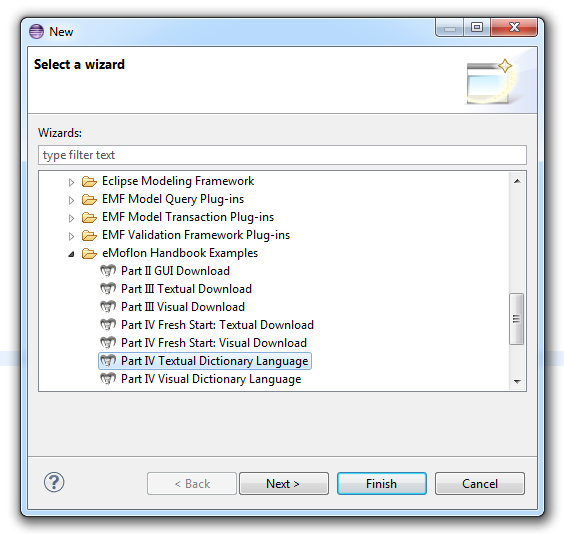
\includegraphics[width=0.8\textwidth]{eclipse_part4DictionaryLanguageDownload}
  \caption{Get the textual Dictionary project}
  \label{eclipse:dictionaryDownloadWizard}
\end{center}
\end{figure}

\item[$\blacktriangleright$] If successful, your workspace should resemble Fig.~\ref{eclipse:loadedDictionaryMetamodel}. It would be a good idea to inspect the
metamodel until you feel comfortable with what you'll be working with. This transformation will be focusing on the \texttt{Dictionary} and \texttt{Entry}
EClasses.

\newpage

\begin{figure}[htbp]
\begin{center}
  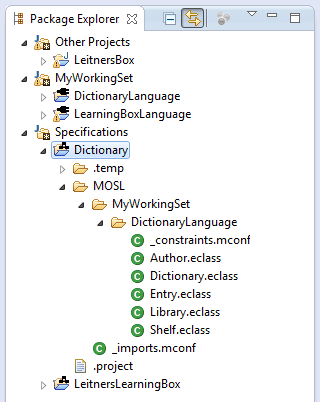
\includegraphics[width=0.5\textwidth]{eclipse_loadDictionaryMetamodel}
  \caption{\texttt{DictionaryLanguage}'s metamodel structure}
  \label{eclipse:loadedDictionaryMetamodel}
\end{center}
\end{figure}

\item[$\blacktriangleright$] While you now have your source and target metamodels, \texttt{Leit\-ners\-Learn\-ing\-Box} is in a different metamodel project
(MOSL folder) and still needs to be allowed to access \texttt{Dict\-ion\-ary\-Lang\-uage}. Navigate to ``LeitnersLearningBox/MOSL/MyWorkingSet,'' open
\texttt{\_imports.mconf} and add the statement \texttt{import Dictionary} (Fig.~\ref{eclipse:importConfigFile}).

\vspace{0.5cm}

\begin{figure}[htbp]
\begin{center}
  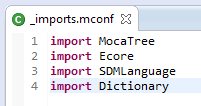
\includegraphics[width=0.35\textwidth]{eclipse_learningBoxImportFile}
  \caption{Importing \texttt{Dictionary} into the learning box}
  \label{eclipse:importConfigFile}
\end{center}
\end{figure}

\item[$\blacktriangleright$] Save and rebuild \texttt{LeitnersLearningBox} by pressing ``Build (without cleaning)'' on the toolbar. You're now ready to start
your TGG!

\end{itemize}
